% In 2022 umgeschrieben, da sich kaum einer mehr ans Diplom erinnert. Fokus jetzt mehr auf Ba-Ma-System anstatt Historie.
\section{Das Bachelor-Master-System im Schnelldurchlauf}

\begin{multicols}{2}
\begin{quote}
	\textit{\foreignlanguage{english}{I accept chaos, I'm not sure whether it accepts me.}}

	\hfill--- Bob Dylan
\end{quote}
Bevor wir euch die einzelnen Physikstudiengänge im Detail vorstellen, soll es hier um den allgemeinen Studienaufbau mit Bachelor- und Masterabschlüssen gehen.
Eingeführt wurde das heutige System durch den Bologna-Prozess seit der Jahrtausendwende und ersetzte damit das Diplomstudium. Wer im eigenen Umfeld Bekannte hat, die schon vorher ein Studium abgeschlossen haben, kann sicherlich einige nostalgische Geschichten zu den Vor- und Nachteilen des Diploms von diesen zu hören bekommen.
Das Bachelor-Master-System sollte vor allem zu einer europaweiten Vereinheitlichung und Vergleichbarkeit führen.

\textbf{Wichtige Ziele der Deklaration:}
\begin{itemize}
	\item die Schaffung eines Systems leicht verständlicher und vergleichbarer Abschlüsse
	\item Förderung der Mobilität (Erasmus, Erasmus+)
	\item Förderung der europäischen Zusammenarbeit im Bereich der Qualitätssicherung
\end{itemize}

Natürlich stellte diese Reform zunächst eine große Veränderung für die Hochschulen dar und kam nicht ohne Kritik aus. Mittlerweile hat sich das System in Deutschland etabliert, was aber keinesfalls heißen soll, dass nun alles perfekt ist. Das Studium besteht jetzt aus einem Bachelor, der in Deutschland in der Regel 3 Jahre dauert und 180 Creditpoints/Leistungspunkte umfasst, und einem abschließenden Master von 2 Jahren und 120 Leistungspunkten. Die Leistungspunkte gibt es am Ende sogenannter Module, in denen Vorlesungen, Übungen, Seminare etc. zu einem Thema zusammengefasst sind und die mit einer Modulabschlussprüfung beendet werden. Am Ende steht noch eine Bachelor- oder Masterarbeit, die euch dann den entsprechenden berufsqualifizierenden Abschluss einbringt. 

Nach anfänglichen Schwierigkeiten, zu denen noch die Einführung elektronischer Prüfungssysteme wie dem QISPOS beigetragen haben, lässt sich mittlerweile ein erstes Fazit zum Bachelor-Master-System ziehen:
Als besonders positiv hat sich die hohe Anrechenbarkeit von international absolvierten Credits gezeigt, was insbesondere in der gestiegenen Anzahl an absolvierten Auslandsaufenthalten deutlich wird. Zudem ist durch die Zweistufigkeit ein Wechsel nach dem Bachelor in einen anderen Master leicht möglich und durch die Modularisierung konnten neue spezifizierte Studiengänge angeboten werden. Insbesondere bei Physik lässt dies einen hohen Grad an Spezial-Mastern zu, sofern genügend Masterplätze zur Verfügung stehen.
Als Kritikpunkt wird oft angeführt, dass durch die strikten Modulvorgaben die individuelle Entfaltung der Studierenden zu kurz kommt und auch der Bachelor ist in der Physik praktisch nicht wirklich berufsqualifizierend - Meist ist der anschließende Masterabschluss notwendig. Auch die Arbeitsbelastung im Bachelor-Master-System wird regelmäßig kritisiert.

Es gibt also durchaus noch Verbesserungsbedarf und es bleibt zu hoffen, dass die Diskussion über die Bologna-Reformen weiterlebt und in Zukunft weitere Veränderungen erzielt werden können. Wenn du vielleicht sogar deine eigene Stimme in die Diskussion einfliessen lassen möchtest, ist der Artikel zur Studentischen Mitbestimmung etwas weiter hinten in dieser Fibel empfehlenswert. 

\fibelsig{Moritz}

\vspace{3ex}

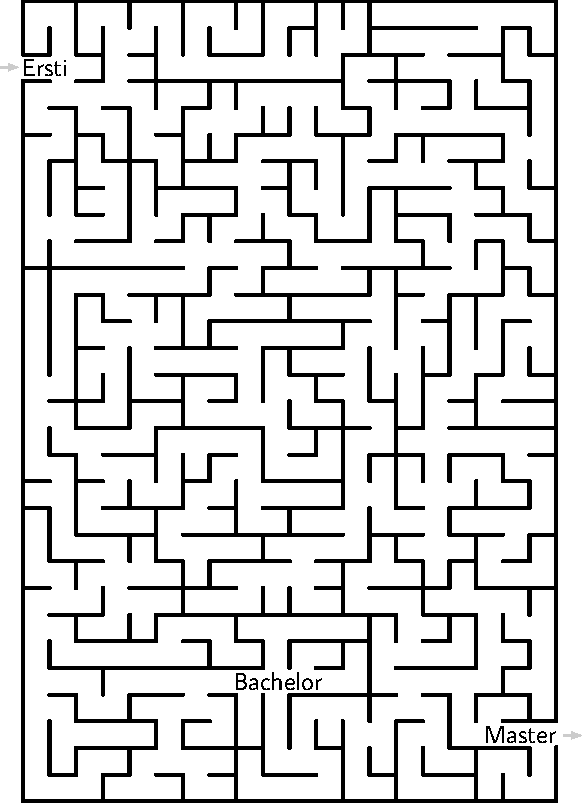
\includegraphics[width=\columnwidth]{res/bachelor_master_labyrinth.pdf}
\end{multicols}
